
\documentclass[11pt]{article}
\usepackage{latexsym}
\usepackage{amsmath}
\usepackage{amssymb}
\usepackage{amsthm}
\usepackage{epsfig}
\usepackage{lipsum}
\usepackage{graphicx}
\usepackage{algorithm,float}
%\usepackage{algorithmic}
\usepackage[noend]{algpseudocode}
\usepackage{algorithm}% http://ctan.org/pkg/algorithms
\MakeRobust{\Call}
%\theoremstyle{definition}
\newtheorem{exmp}{Example}[section]

\newcommand{\handout}[5]{
  \noindent
  \begin{center}
  \framebox{
    \vbox{
      \hbox to 5.78in { {\bf ICS 621: Analysis of Algorithms } \hfill #2 }
      \vspace{4mm}
      \hbox to 5.78in { {\Large \hfill #5  \hfill} }
      \vspace{2mm}
      \hbox to 5.78in { {\em #3 \hfill #4} }
    }
  }
  \end{center}
  \vspace*{4mm}
}

\newcommand{\lecture}[4]{\handout{#1}{#2}{#3}{Scribe: #4}{Lecture #1}}

\newtheorem{theorem}{Theorem}
\newtheorem{corollary}[theorem]{Corollary}
\newtheorem{lemma}[theorem]{Lemma}
\newtheorem{observation}[theorem]{Observation}
\newtheorem{proposition}[theorem]{Proposition}
\newtheorem{definition}[theorem]{Definition}
\newtheorem{claim}[theorem]{Claim}
\newtheorem{fact}[theorem]{Fact}
\newtheorem{assumption}[theorem]{Assumption}

% 1-inch margins, from fullpage.sty by H.Partl, Version 2, Dec. 15, 1988.
\topmargin 0pt
\advance \topmargin by -\headheight
\advance \topmargin by -\headsep
\textheight 8.9in
\oddsidemargin 0pt
\evensidemargin \oddsidemargin
\marginparwidth 0.5in
\textwidth 6.5in

\parindent 0in
\parskip 1.5ex
%\renewcommand{\baselinestretch}{1.25}
% for whole paragraph indent
\newenvironment{myindentpar}[1]%
  {\begin{list}{}%
          {\setlength{\leftmargin}{#1}}%
          \item[]%
  }
  {\end{list}}




\begin{document}

\lecture{8}{Fall 2019}{Prof.\ Nodari Sitchinava}{Mojtaba Abolfazli, Honggen Zhang}

% \section{Overview}
\section{Introduction}
This session is the continuation of the last session on randomized search trees where we are interested to dive deeper into the analysis of treaps and skip lists. Before going into detail, we need to recall important results of the last session:
\begin{itemize}
    \item The expected time for search for treaps is of the order $\mathcal{O}(\log n)$.
    \item The height of skip lists is of the order $\mathcal{O}(\log n)$ with high probability.
    \item In a skip list, the probability that the key $x$ appears on the level $l$ is:
    \begin{equation}\label{eq:prob-greater}
        Pr[L(x) \geq l] = \frac{1}{2^l}
    \end{equation}
    It's equivalent to the experiment of repeatedly flipping a coin and having it come up \Call{heads}{} $l$ times in a row when we insert $x$.
    \item For any constant $c>1$, we also have the following bound for skip lists:
    \begin{equation*}
      Pr[\max\limits_{x} \{L(x)\} \geq (c+1)\log n ] \leq \frac{1}{n^c}.  
    \end{equation*}
\end{itemize}

\section{Skip Lists}
\subsection{Expected Number of Levels}
Before showing the expected number of levels in the skip lists, we need to introduce a lemma.
\begin{lemma}\label{lemma1:expec}
For any non-negative integer random variable $X$:
\begin{equation*}
    \mathbb{E}[X] = \sum_{x=1}^{\infty} Pr[X \geq x]
\end{equation*}
\end{lemma}

Before we prove Lemma~\ref{lemma1:expec}, first, let us prove a simple fact about summations:

\begin{lemma}\label{lemma:sums}
$$\sum_{x=1}^n x \cdot f(x) = \sum_{x=1}^n\sum_{k=x}^n f(k)$$
\end{lemma}
\begin{proof}
  
\begin{align*}
    \sum_{x=1}^n x \cdot f(x) &= 1\cdot f(1) + 2\cdot f(2) + \dots n\cdot f(n) \qquad \mbox{Rearranging the terms, we get:} \\
    &= \Big( f(1) + f(2) + f(3) + \dots + f(n)\Big) + \Big( f(2) + f(3) + \dots f(n)\Big) + \dots + \Big(f(n)\Big) \\
 %&= \Big(f(1)\Big) + \Big(f(2)+f(2)\Big) + \Big(f(3)+f(3)+f(3)\Big) + \dots + \Big(f(n)+ f(n) + \dots + f(n) + f(n)\Big) \\
  &= \sum_{k=1}^n f(k) + \sum_{k=2}^n f(k) + \dots + \sum_{k=n}^n f(k) \\
%n\cdot f(1) + (n-1)\cdot f(2)+ \dots + 2\cdot f(n-1) + 1\cdot f(n)\\
  %&= \sum_{x=1}^n \sum_{k=x}^n (n-x+1) \cdot f(x) \\
  &= \sum_{x=1}^n \sum_{k=x}^n f(k)  \qedhere
\end{align*}
\end{proof}

Now we are ready to prove Lemma~\ref{lemma1:expec}.
\begin{proof}[Proof of Lemma~\ref{lemma1:expec}]
Recall that $\mathbb{E}[X] = \sum\limits_{x=1}^\infty x\cdot Pr[X=x]$. Then by using the function $f(x) = Pr[X=x]$ and setting $n = \infty$ in Lemma~\ref{lemma:sums} we get:
\begin{align*}
     \mathbb{E}[X] = \sum_{x=1}^\infty x\cdot Pr[X=x]
      = \sum_{x=1}^{\infty} \sum_{k=x}^\infty Pr[X=k]  
\end{align*} 

Now observe that by the definition of probabilities 
$$\sum\limits_{k=x}^\infty Pr[X=k] =  Pr[X \geq x] $$
and the lemma follows.
\end{proof}
Based on Lemma \ref{lemma1:expec} and by defining $L = \max\limits_{x} \{L(x)\} $, we have:
\begin{align*}
    \mathbb{E}[L] &= \sum_{l=1}^{\infty} Pr[L \geq l]\\
    &= \sum_{l=1}^{\log n} Pr[L \geq l] + \sum_{l=\log n +1}^{\infty} Pr[L \geq l]\\
\end{align*}

Observe that any probability is at most $1$, i.e. $Pr[L\ge l] \le 1$, which will be sufficient for the first term above. To bound the second term, we can prove a tighter bound on $Pr[L\ge l]$ using the Union Bound: 

\begin{align*}
  Pr[L \geq l] & = Pr[L(x_1) \vee \ldots \vee L(x_n)] \\
  & \leq \sum_{i=1}^{n}Pr[L(x_i) \geq l)] & \mbox{By equation (\ref{eq:prob-greater}):}\\
  & = \sum_{i=1}^{n} \frac{1}{2^l} \\
  &=  \frac{n}{2^l}
\end{align*}
Then:
\begin{align*}
    \mathbb{E}[L] &= \sum_{l=1}^{\log n} Pr[L \geq l] + \sum_{l=\log n +1}^{\infty} Pr[L \geq l]\\
    & \leq  \sum_{l=1}^{\log n} 1 + \sum_{l = \log n +1}^{\infty} \frac{n}{2^l}\\
    & = \log n + \sum_{i=1}^{\infty} \frac{n}{2^{\log n + i}}\\
    & = \log n + \sum_{i=1}^{\infty} \frac{n}{n \cdot 2^i}\\
    &= \log n + 1
\end{align*}

I.e., the expected number of levels of a skip list is one more than the ideal case where each level contains exactly half the nodes of the level below.

\subsection{Search Time}
Let us analyze the expected cost of a search in a skip list. This is proportional to the number of elements that the search algorithm will visit. To simplify this computation, consider the sequence of elements that the search algorithm will visit and let us trace this path in the backward direction from the search destination at the bottom of the data structure to the root (see Figure~\ref{fig:backward} for an illustration). Tracing the algorithm from the search destination node $v$ at the bottom of the level of the data structure is equivalent to the following algorithm:

\begin{algorithm}[H]
\caption{An equivalent algorithm for backward tracing of a search}\label{skiplist1}
\begin{algorithmic}[1]
\Function{Backward-Search}{$v$}
\While{$v \neq root$}
    \If {$up(v) \neq NIL$}
    \State $v=up(v)$
    \Else 
    \State $v = left(v)$
    \EndIf
\EndWhile
\EndFunction
\end{algorithmic}
\end{algorithm}
For every node $v$ in the skip list, the link $up(v)$ exists if the coin flip came up \Call{heads}{} during the insertion of $v$. Thus, it exists with probability $\frac{1}{2}$. From the analysis perspective, this is exactly like the following algorithm in which we flip a fair coin during the backward traversal.

\begin{algorithm}[H]
\caption{An equivalent algorithm for Backward tracing of a search via coin flipping}\label{skiplist2}
\begin{algorithmic}[1]
\Function{Backward-Search-Flip}{$v$}
\While{$v \neq root$}
    \If {$\Call{coinFlip}{\null} == \Call{heads}{}$}
    \State $v=up(v)$
    \Else 
    \State $v = left(v)$
    \EndIf
\EndWhile
\EndFunction
\end{algorithmic}
\end{algorithm}
For the above algorithm, we have the same expected number of \Call{tails}{} and \Call{heads}{} since we flip a fair coin. Therefore, the expected running time of search, $\mathbb{E}[T]$, is twice the expected number of times of going upward in the tree (the height of the tree $L$):
\begin{equation*}
    \mathbb{E}[T] = \mathbb{E}[2L] \leq 2(\log n +1) = O(\log n)
\end{equation*}

\begin{figure}[H]
\begin{center}
    
  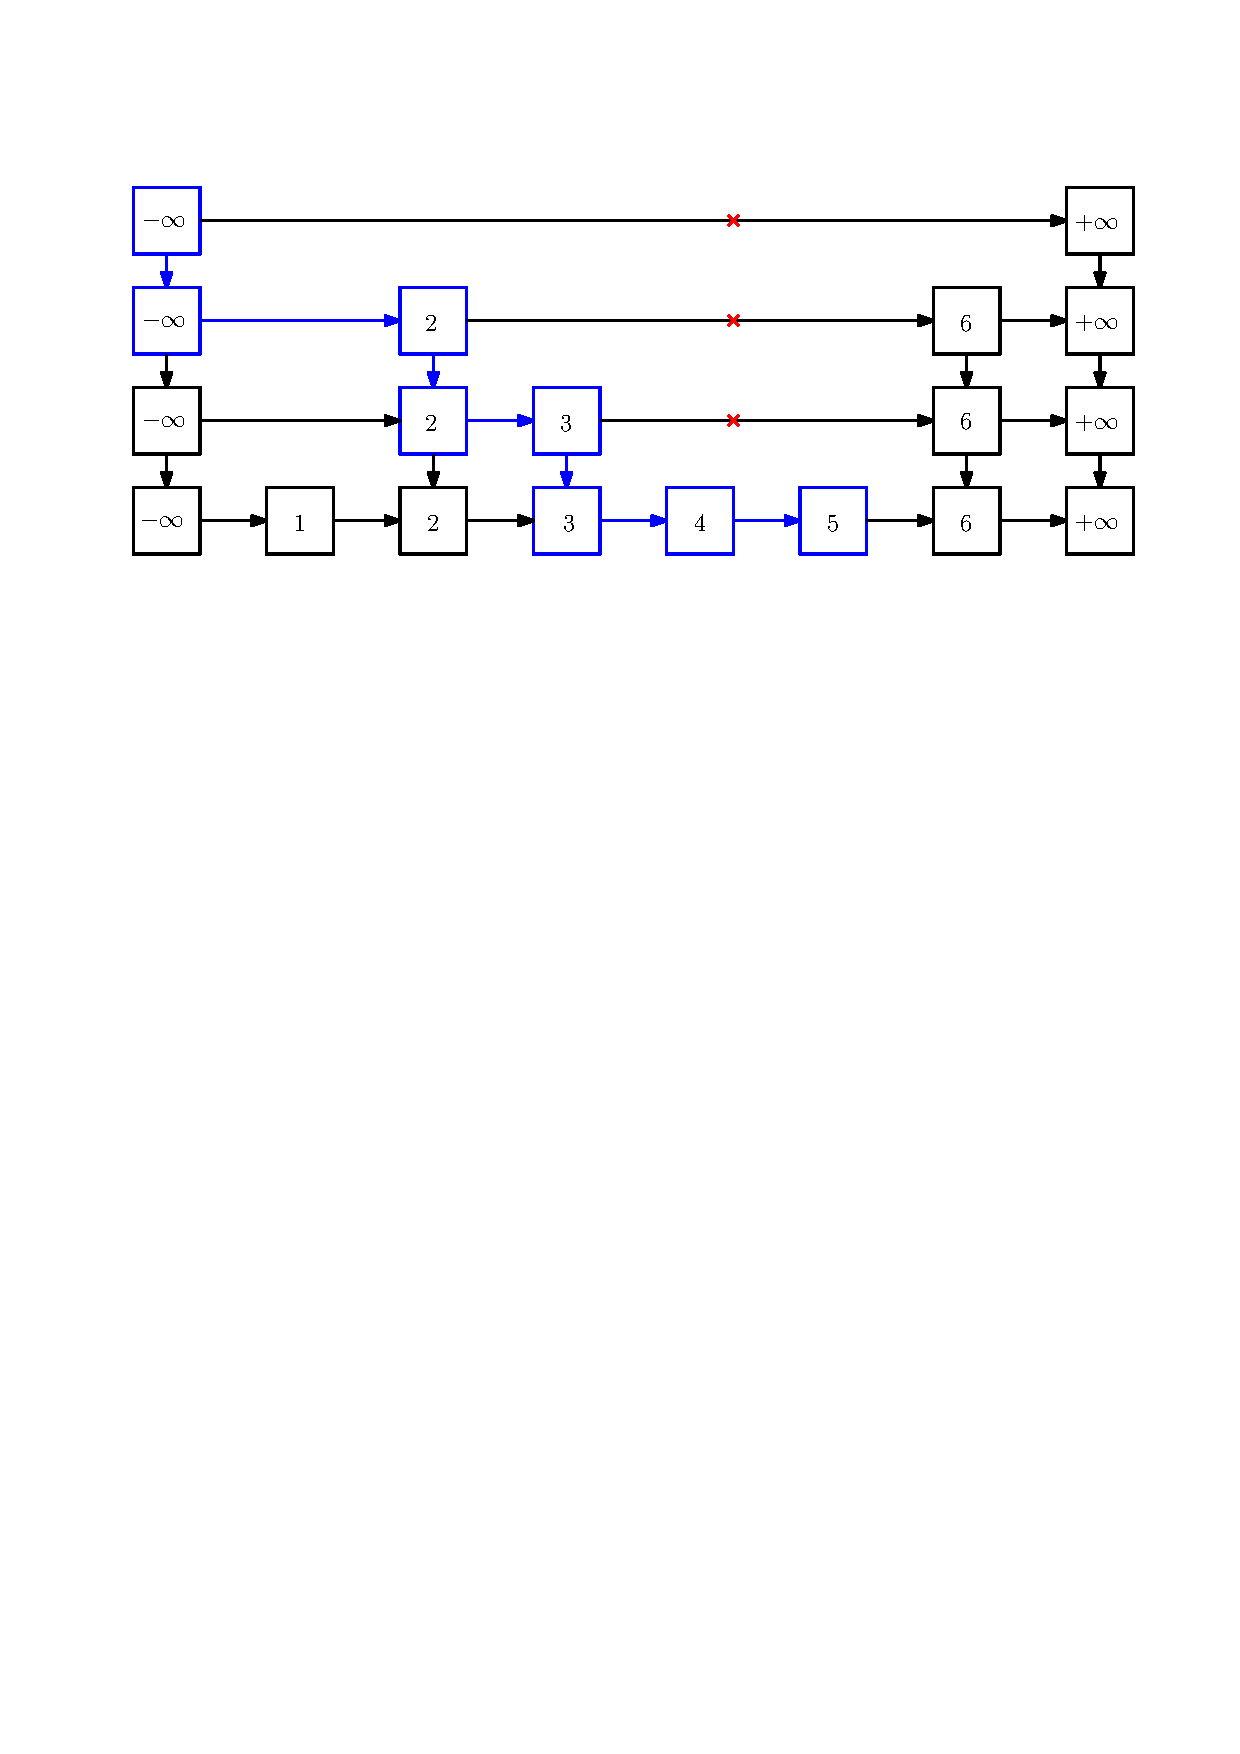
\includegraphics[width=5in]{searchTreaps.pdf}
  \vspace{-0.1in}
  \caption{\label{search.fig}Searching for 5 in a skip list.}
  \label{fig:backward}
\end{center}
\end{figure}



\section{Treaps}
In order to analyze the performance of treaps, we need to use some sort of approximations. In this part, we explore some elementary techniques on tail distributions. It is worth mentioning that they provide good approximations on deviation and concentration of random variables.

\subsection{Markov's Inequality}
It is the most elementary tail bound which is defined for a non-negative random variable with finite mean as follows:
\begin{equation*}
    Pr[X \geq a] \leq \frac{\mathbb{E}[X]}{a}
\end{equation*}
\begin{proof}
 We can use Lemma \ref{lemma1:expec} to prove this inequality:
\begin{align*}
    \mathbb{E}[X] &= \sum_{x=0}^{a-1} x \cdot Pr[X=x] + \sum_{x=a}^{\infty} x \cdot Pr[X=x]\\
    &\geq \sum_{x=a}^{\infty} x \cdot Pr[X=x]\\
    & \geq a \sum_{x=a}^{\infty} Pr[X=x]\\
    & = a Pr[X \geq a]
\end{align*}
by rearranging the terms:
    $$Pr[X \geq a] \leq \frac{\mathbb{E}[X]}{a} \qedhere$$ 
\end{proof}

\subsection{The Height of Treaps}
Now, we want to apply Markov's inequality to treaps and see for what values of $h$, the following inequality holds:
\begin{equation*}
    Pr[\Call{Height}{Treap} \geq h] \leq  \frac{1}{n}
\end{equation*}
The height of a treap is greater than or equal to $h$ the height of at least one node in the treap is greater than or equal to $h$, i.e.:
\begin{equation*}
    Pr[\Call{Height}{x_1} \geq h \vee \Call{Height}{x_2} \geq h \vee \ldots  \vee \Call{Height}{x_n} \geq h] \leq  \frac{1}{n}
\end{equation*}
The \textbf{union bound} states that the probability that at least one of the events happens is no greater than the sum of the probabilities of the individual events. Therefore, we can find an upper bound based on $x_k$ as the node with the $k$th smallest search key:
\begin{align*}
    n \cdot Pr[\Call{Height}{x_k} \geq h] \leq \frac{1}{n} \hspace{0.2cm}\Rightarrow \hspace{0.2cm} Pr[\Call{Height}{x_k} \geq h] \leq \frac{1}{n^2}  
\end{align*}

by applying Markov's inequality:

\begin{equation*}
Pr[\Call{Height}{x_k} \geq h] \leq \frac{\mathbb{E}[X]}{h} = \frac{\log n}{h} \leq \frac{1}{n^2}   
\end{equation*}

which gives $h \geq n^2\log n$. As we know, the height of a treap with $n$ elements cannot be greater than $n$. Thus, the resulting condition for $h$ is not useful. To conclude, the Markov's inequality does not give a tight bound on the value of the height. In the rest, we'll introduce tighter bounds, which provide useful information about the tree structure.

\subsection{Chebyshev's inequality}
Chebyshev's inequality is a probabilistic inequality. It provides an upper bound to the probability of the absolute deviation between the random variable and its mean.
\begin{definition}
Two random variables $X,Y$ are independent iff
\[
Pr[(X=x) \wedge (Y=y)]=Pr[X=x]\cdot Pr[Y=y]
\]
for all possible values $x,y$.
\end{definition}
\begin{definition}
Set of random variables $X_1,X_2,\ldots,X_n$ are $k$-wise independent if every subset of $k$ variables is independent.
\end{definition}
\begin{corollary}
If $X_1,X_2,\ldots,X_n$ are $k$-wise independent, then for any integer $2\le k^\prime <k$, they are also $k^\prime$-wise independent.
\end{corollary}
\begin{theorem}
Let $X_1,X_2,\ldots,X_n$ be pairwise independent and identical random variables and $X=\sum_{i=1}^n X_i$ with $\mathbb{E}[X]=\mu$, then
\[
Pr[(x-\mu)^2 \ge a]<\frac{\mu}{a},
\]
for any $a>0$.\
\end{theorem}
When $a=k^2$
\[
Pr[(x-\mu)^2 \ge k^2]<\frac{\mu}{k^2}.
\]
Because $(x-\mu)^2 \ge k^2$, we have $|x-\mu|\ge k$ and therefore:
\[
Pr[|x-\mu)| \ge k]<\frac{\mu}{k^2}.
\]

By setting $\Delta=k$, we get the {\em additive} tail bounds:

\[Pr[x\ge \mu+\Delta]\leq \frac{\mu}{\Delta^2}, \quad  Pr[x\leq \mu-\Delta]\le \frac{\mu}{\Delta^2}\]

By setting $\delta\mu=k$, we get the {\em multiplicative} tail bounds:

\[Pr[x\ge (1+\delta)\mu]\leq \frac{1}{\delta^2\mu}, \quad  Pr[x\leq (1-\delta)\mu]\leq \frac{1}{\delta^2\mu}.\]

\subsubsection{Higher Moment Inequality}
\begin{theorem}
For any fixed integer $k>0$, if $X_1,X_2\ldots X_n$ are $2k$-wise independent and $X=\sum_{i=1}^n X_i$, then
\[
Pr[(X-\mu)^k\ge a]\leq \mathcal{O} \left(\frac{\mu^k}{a}\right).
\]
\end{theorem}
\begin{corollary}
The additive bounds:
\[
Pr[X\ge \mu+\Delta]=\mathcal{O} \left(\left(\frac{\mu}{\Delta^2}\right)^k\right)
,\ \ Pr[X\leq \mu-\Delta]=\mathcal{O} \left(\left(\frac{\mu}{\Delta^2}\right)^k\right) .
\]
The multiplicative bounds:
\[
Pr[X\ge (1+\delta)\mu]=\mathcal{O} \left(\left(\frac{1}{\delta^2\mu}\right)^k\right) ,\ \ Pr[X\leq (1-\delta)\mu]=\mathcal{O} \left(\left(\frac{1}{\delta^2\mu}\right)^k\right).
\]
\end{corollary}

\subsection{Chernoff bound}
Markov's inequality requires the random variable to be non-negative. Therefore, in order to use Markov's inequality, it is necessary to modify the original random variable and construct a function of the random variable, which can only take non-negative values. The most common non-negative functions are even power functions and exponential functions.
The Chernoff bound uses exponential functions.
\begin{theorem}
If identical random variables $X_1,X_2,\ldots,X_n$ are fully independent, then for all $a\ge \mu$, $X=\sum_{i=1}^n X_i$:
\[
Pr[X\ge a]\leq e^{a-\mu}\left(\frac{\mu}{a}\right)^a.
\]
\end{theorem}
\begin{corollary}
The additive tail bounds:
\[
Pr[X\ge \mu+\Delta]\leq e^\Delta \left(\left(\frac{\mu}{\mu +\Delta}\right)^{\mu+\Delta}\right),
\ \ Pr[X\leq \mu-\Delta]\leq e^{-\Delta}\left(\left(\frac{\mu}{\mu +\Delta}\right)^{\mu+\Delta}\right),
\]
The multiplicative tail bounds:
\[Pr[X\ge (1+\delta)\mu] \leq
 \left(\frac{e^\delta}{(1+\delta)^{1+\delta}}\right)^\mu ,\ \ Pr[X\leq (1-\delta)\mu] \leq
 \left(\frac{e^{-\delta}}{(1-\delta)^{1-\delta}}\right)^\mu.
\]
When $0<\delta<1$, the Chernoff multiplicative bound can be simplified as:
\[
Pr[X\ge (1+\delta)\mu] \leq e^{\frac{-\delta^2\mu}{3}},\ \Pr[X\leq (1-\delta)\mu]  \leq e^{\frac{-\delta^2\mu}{2}}
\]
This simple form of Chernoff bound is easier to use, but we should notice that they provide probability with looser bounds.
\end{corollary}
\begin{exmp}
We flip a fair coin $N$ times. Let $X$ be a random variable, which represents the number of \Call{heads}{}. What is the probability that $Pr\left[X\ge \frac{3N}{4}\right]$?
\end{exmp}
Let us compute $Pr[X \ge aN]$ for any $a> 0$. 

We know that $\mu=\frac{N}{2}$. Thus, $aN = 2a\mu = (1+\delta)\mu$ for $\delta = 2a-1$. %Then $Pr[X \ge aN] = Pr[X \ge ]$
%\[
%Pr[X\ge \frac{3N}{4}]=Pr[X\ge \frac{3\mu}{2}]
%\]
By using Chernoff's bound for $\delta = 2a-1$ we get:
\[
Pr[X\ge aN] = Pr[X\ge (1+(2a-1))\mu] \leq e^{-\frac{(2a-1)^2 \mu}{3}} = e^{-\frac{(2a-1)^2 N}{6}} 
\]

And by using $a = 3/4$ we get $Pr\left[X \ge \frac{3N}{4}\right] \le e^{-\frac{N}{24}}$
\subsection{Height Analysis}
\begin{theorem}
The expected height of the treap is $\mathcal{O}(\log n)$.
\end{theorem}
\begin{proof}
Let ${x_1,x_2,\ldots,x_n}$ be the order of keys in the treap and let $Y_{i,j}$ be an indicator random variable that takes 1 if $x_i$ is the proper ancestor of $x_j$. Last week we showed that $Y_{i,j}=1$ iff $x_i$ has the smallest priority in the range $[x_i,\ldots, x_j]$. I.e., $Pr[Y_{i,j} = 1] = \frac{1}{|i-j|+1}$ for any $i \ne j$ and $Y_{i,i}$ is always $0$ for all $i$. Then the height of any node $x_k$  can be determined as

\[\Call{Height}{x_k}=\sum_{i=1}^n Y_{i,k}=\sum_{i=1}^{k-1} Y_{i,k}+\sum_{i=k+1}^n Y_{i,k}\]

By the linearity of expectations: 
\[
\mathbb{E}[\Call{Height}{X_k}]=\mathbb{E}\left[\sum_{i=1}^n Y_{i,k}\right]=\sum_{i=1}^{k-1} \mathbb{E}[Y_{i,k}]+\sum_{i=k+1}^n \mathbb{E}[Y_{i,k}].
\]
 Since the expectation of an indicator random variable is equal to its probability of being equal to $1$, we get:
 \[
 \mathbb{E}[\Call{Height}{X_k}]=\sum_{i=1}^{k-1} Pr[Y_{i,k}=1]+\sum_{i=k+1}^n Pr[Y_{i,k}=1]
 \]
\[
=\sum_{i=1}^{k-1} \frac{1}{k-i+1} +\sum_{i=k+1}^n \frac{1}{i-k+1}.
\]
By changing the indices of the summations: 
\begin{align*}
\mathbb{E}[\Call{Height}{X_k}]&=\sum_{t=2}^{k} \frac{1}{t} +\sum_{t=2}^{n-k} \frac{1}{t} \\
&=\sum_{t=2}^{k} \frac{1}{t} +\sum_{t=2}^{n-k} \frac{1}{t} \\
&\leq (H_k-1)+(H_{n-k}-1)\\
&\leq 2H_n -2
\end{align*}
Where $H_n$ is the $n$th Harmonic number:
\[
H_n=\sum_{i=1}^n\frac{1}{i}=\ln{n}+\mathcal{O}(1)
\]

Thus, $\mathbb{E}[\Call{Height}{X_k}] \le 2\ln n -2 = 2\ln n + \mathcal{O}(1) = \mathcal{O}(\log n)$, i.e., the expected height of a treap is $\mathcal{O}(\log n)$.
\end{proof}
To analyze the height of a treap with high probability, we will use Chernoff bound. However, to use it, we need the following lemma about indepence of random variables $Y_{i,j}$.
\begin{lemma}
For every $k\in\{1,2,\ldots,n\}$, the indicator random variables $Y_{1,k},Y_{2,k},\ldots,Y_{k-1,k}$ are mutually independent. Similarly, the indicator random variables  $Y_{k+1,k},Y_{k+2,k},\ldots,Y_{n,k}$ are mutually independent.
\end{lemma}
\begin{proof}
We will consider only the set of indicator random variables  $\{Y_{i,k}\}$ with $i > k$. The proof for the set $\{Y_{i,k}\}$ for $i < k$ is similar.
To simplify notation, let $X_i$ denote the indicator variable $Y_{i,k}$.

The proof is by induction on the number of variables $Y_{i,k}$ with the inductive hypothesis that $ Y_{k+1,k},Y_{k+2,k},\ldots,Y_{n-1,k}$ are mutually independent. 

Given the above hypothesis, let us prove that $Y_{k+1,k},Y_{k+2,k},\ldots,Y_{n,k}$ are mutually independent. Since $Y_{i,k}$ are indicator random variables, let $y_i = \{0,1\}$ be the values that $Y_{i,k}$ may take. Recall that 
$$Pr[(A = a) \wedge (B= b)] = Pr[(A = a) \mid (B=b)] \cdot Pr[B = b],$$ 
where $Pr[(A = a) \mid (B = b)]$ denotes the ``conditional probability that $A = a$, given $B = b$". Then
\[
Pr\left[\bigwedge_{i=k+1}^{n} (Y_{i,k}=y_i)\right]=Pr\left[\left(\bigwedge_{i=k+1}^{n-1} (Y_{i,k}=y_i)\right)\wedge (Y_{n,k}=y_n)\right]
\]
\[
=Pr\left[\left(\bigwedge_{i=k+1}^{n-1} (Y_{i,k}=y_i)\right)\mid(Y_{n,k}=y_n)\right]\cdot Pr[Y_{n,k}=y_n]
\]
Since $Y_{n,k}=1$ iff node $x_n$ has the smallest priority among the nodes $x_{k+1}, \ldots, x_n$, the other indicator variables $Y_{k+1,k}, \ldots, Y_{n-1,k}$ only depend on the order of the priorities among the nodes with keys $x_{k+1}, \ldots, x_{n-1}$. Therefore:
\[
Pr\left[\left(\bigwedge_{i=k+1}^{n-1} (Y_{i,k}=y_i)\right)\mid(Y_{n,k}=y_n)\right]=Pr\left[\bigwedge_{i=k+1}^{n-1} (Y_{i,k}=y_i)\right]
\]
By the inductive hypothesis, variables $Y_{k+1,k},Y_{k+2,k},\ldots,Y_{n-1,k}$ are mutually independent, i.e., 
\[
Pr\left[\bigwedge_{i=k+1}^{n-1} (Y_{i,k}=y_i)\right]=\prod_{i=k+1}^{n-1} Pr[Y_{i,k}=y_i]
\]
We conclude that:
\[
Pr\left[\bigwedge_{i=k+1}^{n} (Y_{i,k}=y_i)\right]=\prod_{i=k+1}^{n-1} Pr[Y_{i,k}=y_i]\cdot Pr[Y_{n,k}=y_n]=\prod_{i=k+1}^{n} Pr[Y_{i,k}=y_i] 
\]

I.e., indicator random variables $Y_{k+1,k}, \ldots, Y_{n,k}$ are mutually independent.
\end{proof}
\end{document}
